\documentclass[a4paper,10pt]{scrartcl}
\usepackage[utf8]{inputenc}
\usepackage[hyphens]{url}
\usepackage{hyperref}
\usepackage[ngerman]{babel}
\usepackage[T1]{fontenc}
\usepackage{graphicx}
\usepackage[utf8]{inputenc}
\usepackage{lmodern}
\usepackage{geometry}
\usepackage{pgfplots} 
\usepackage{mathrsfs}
\usepackage{mathtools}
\usepackage{listings}
\usepackage{wrapfig}
\usepackage{float}
\usepackage{amsmath}
\usepackage{stmaryrd}
\usepackage{paralist}
\lstset{basicstyle=\normalfont\ttfamily,breaklines=true}


\geometry{paper=a4paper, left=20mm, right=20mm, top=30mm, bottom=30mm}
\hypersetup{
    unicode=false,
    pdftoolbar=true,
    pdfmenubar=true,
    pdffitwindow=false,
    pdfstartview={FitH},
    pdftitle={DataScienceReport},
    pdfauthor={PaSeDa},
    pdfsubject={Subject},
    pdfcreator={Creator},
    pdfproducer={Producer},
    pdfkeywords={keyword1} {key2} {key3},
    pdfnewwindow=true,
    colorlinks=false,
    linkcolor=red,
    citecolor=green,
    filecolor=magenta,
    urlcolor=cyan
}

\title{\vspace{-2cm}Bericht DataSciece Projekt}
\subtitle{Verbindung von Gehalt und Wahlverhalten in Frankfurt}
\author{PaSeDa}
\date{}

\usepackage{etoolbox}


%Mathepakete
\usepackage{amsfonts}
\usepackage{amsmath}
\usepackage{amssymb}
\usepackage{amsthm}    

\newcommand{\TODO}{\textcolor{red}{\textbf{TODO }}}

\allowdisplaybreaks
\begin{document}
\maketitle

\begin{abstract}Dies ist die finale Ausarbeitung unseres Projektes für das Modul DataScience1. Untersucht wurde der Zusammenhang von Gehalt und Wahlverhalten in Frankfurt. Dazu wurden zwei Datensätze  von \TODO verwendet die Informationen von Gehalt und Wahlverhalten je Stadtteil zu Verfügung stellen. Organisiert haben war unser Projekt mit Jupyter Notebooks uns GitHub. Die gesäuberten Datensätze wurden auf verschiedene Weise untersucht. Insbesondere wurden mehrere Multi-Target-Regressoren trainiert, um festzustellen ob eine Wahlvorhersage aufgrund des Gehalts sinnvolle Ergebnisse liefert. Festgestellt haben wir, dass es einen statistisch signifikanten Zusammenhang zwischen Verteilung Gehalt eines Stadtteils und den Wählerstimmen für SPD, FDP und AFD gibt.  \end{abstract}

\tableofcontents

\section{Zielsetzung}
Dass das Wahlverhalten von Deutschen durch ihre Einkommen beeinflusst würde, ist etwas dass viele schon gehört haben oder auch selber vermuten. Wir wollen diese Vermutung an Hand von Daten aus Frankfurt untersuchen.

\section{Unsere Infrastruktur}
Unser gesamtes Projekt ist auf \href{Github}{\lstinline|https://github.com/5yntek/DataScienceProject|} zu finden. Die verwendeten Rohdaten sind unter \lstinline|/data| gesammelt. \TODO \emph{Infrastruktur säubern und hier aufführen}. Unseren Code haben wir in Jupyter Notebooks gesammelt. Sämtlicher Code ist Python3. Nennenswerte Bibliotheken, die wir verwendet haben sind \href{https://www.scipy.org/}{scipy} (\href{https://numpy.org/}{numpy}, \href{https://pandas.pydata.org/}{pandas}, \href{https://matplotlib.org/}{matplotlib}), \href{https://scikit-learn.org/}{sklearn}, \href{https://seaborn.pydata.org/}{seaborn}  und \href{https://github.com/pandas-profiling/pandas-profiling}{pandas-profiling}.

\TODO \emph{Wie sollen wir Referenzen organisieren?}

\section{Die Daten}
Information über die Gehälter der Frankfurter sind leider recht rar. Die einzigen relevanten Daten haben wir in einem Datensatz zum  \href{https://offenedaten.frankfurt.de/dataset/arbeitsmarkt}{Arbeitsmarkt}
gefunden. Dieser Datensatz ist auf dem Portal \href{https://offenedaten.frankfurt.de}{offenedaten.frankfurt.de} zu finden und erhebt nach eigenen Angaben Daten aus dem Jahr 2011 und 2012. Leider ist die auf der Seite angegebene Quelle veraltet, sodass wir die Daten nicht weiter verifizieren können. Dass die Daten nicht aktueller sind ist zwar Schade, sollte für unser Projekt aber kein Hindernis sein. 

Mehr Daten werden über Wahlergebnisse erhoben. Alleine auf offenedaten.frankfurt gibt es diverse Datensätze zu verschiedenen Wahlen. Für uns am interessantesten erscheinen Daten zur Bundestagswahl, sodass wir uns für den Datensatz der \href{https://offenedaten.frankfurt.de/dataset/bundestagswahl-2017-ergebnisse-in-frankfurt-am-main}{Bundestagswahl 2017} (im weiteren BW17 genannt) entschieden haben.

Leider ist die kleinste Entität, über die Daten sowohl für Gehalt als auch Bundestagswahl erhoben wurde, das Stadtteil, so dass wir mit nur insgesamt \TODO\emph{(wie viele?)} Datenpunkten arbeiten.

Glücklicherweise liegen die Daten sowohl der Bundestagswahl als auch des Arbeitsmarktes in CSV- oder JSON-Dateien vor. Dies erleichtert das Einlesen der Rohdaten in \lstinline|pandas.DataFrames|, der Datenstruktur in der wir intern die Daten repräsentieren und mit der wir arbeiten.

Das Einlesen der Daten findet im Notebook \TODO unter \TODO statt.


\section{Preprocessing}
Ein Blick in die Daten zeigt uns, dass viele Daten fehlen und einige für uns uninteressant sind. Auch sind die Namen der Stadtteile der beiden Datensätze nicht vollständig identisch.

\subsection{Merge and clean the data}
Zunächst verwerfen wir Informationen aus den Rohdaten die wir nicht gebrauchen können \TODO{Referenz}, so zum Beispiel totale Werte. Die Gesamtanzahl der Wähler einer Partei ist nicht interessant, da wir nur relative Werte gebrauche können, um Stadtteile miteinander vergleichen zu können. Weitere Probleme die wir lösen mussten: Wir müssen dafür sorgen, dass numerische Werte richtig interpretiert werden. Die deutsche Variante der Darstellung von Zahlen ist untypisch und muss transformiert werden. Einige Sonderzeichen befinden sich in den Bezeichnern der Attribute, die entfernt werden müssen. Die Attributnamen sind generell unpraktisch lang und werden umbenannt. Die Stadtteile Gutleut- und Bahnhofsviertel wurden in BW17 unter \emph{Gutleut-/Bahnhofsviertel} zusammengefasst und müssen getrennt werden. Die Anteile des Bruttoarbeitsentgelts sind nicht direkt vorhanden und müssen zunächst aus den anderen Daten errechnet werden.
Nach diesen Schritten können wir die beiden Tabellen zusammenführen.

\subsection{Test and verify your data quality}
\TODO Hat jemand eine Idee was genau wir hier schreiben sollen? 

\subsection{Further preprocessing}
\TODO


\subsection{pandas-profiling}
Als ersten Schritt nach dem das Säubern der Daten abgeschlossen ist, ist eine statistische Analyse der Daten. Ein Tool mit dem wir bereits gute Erfahrung gemacht haben ist pandas-profiling. Dieses Framework erzeugt mit wenigen Zeilen einen ausführlichen Bericht in Form von einem HTML-Dokument. Pandas-Profiling zeigt unter anderem fehlende Werte, Datentypen und -Bereiche, sowie Korrelation an. Letztere ist besonders interessant. Pandas-Profling liefert mehrere gut lesbare Diagramme zu Korrelationen innerhalb der Daten. Ein davon stellt die Pearson-Korrelation (r) da. Diese ist ein Maß für die lineare Korrelation zwischen zwei Variablen. Sein Wert liegt zwischen -1 und +1. -1 steht für maximale negative lineare Korrelation, 0 zeigt keine lineare Korrelation an und 1 zeigt maximale positive lineare Korrelation. Abbildung \ref{fig:correlation} stellt die Pearson-Korrelation der Daten da. Einige Zusammenhänge fallen schnell ins Auge, so hat z. B. die FDP eine sehr starke (Anti-)Korrelation zur Gehaltsgruppe 2000-bis-4000. Nicht minder stark (anti-)korreliert das Wahlergebnis der CDU mit dem der DIE LINKE.
\begin{figure}
	\centering
	\fbox{	
		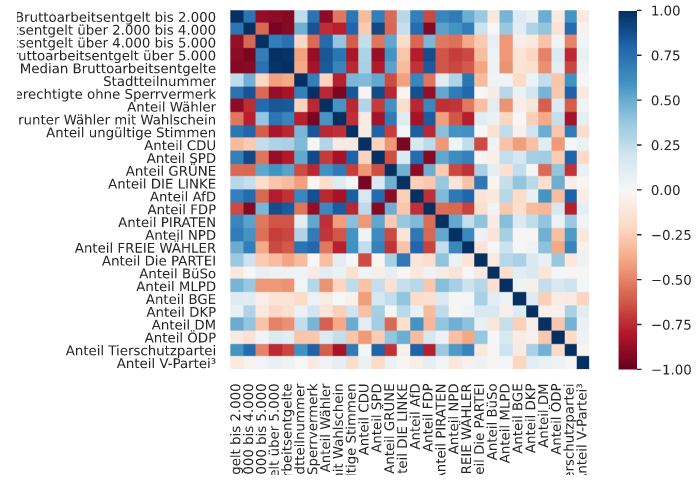
\includegraphics[width=0.8\textwidth]{figure/correlation}
	}
	\caption{Pearson-Korrelation der Daten}
	\label{fig:correlation}
\end{figure}


\section{Apply two different algorithms of the same kind}
Wir haben ein interessantes Problem hier. Wir wollen weder eine Klassifizierung noch eine Regression. Unser gesuchtes Ergebnis ist die Ausprägung(Stimmanteil) verschiedener Parteien(Klassen). Ich denke One-versus-the-rest bzw. Multinomial logistic regression sollten wir auf jeden Fall anwenden.

\section{Evaluate and verify the results of them!}
TODO
\section{Come up with a conclusion!}
TODO
\end{document}
